\documentclass[8pt,a4paper,compress]{beamer}
%\documentclass[8pt,a4paper,compress,handout]{beamer}

\usepackage{amsmath, amssymb, amsthm}
\usepackage{enumerate}
\usepackage{framed}
\usepackage{listings}
\usepackage{tikz}
\usepackage{wrapfig}

\usecolortheme{dove}
\useinnertheme{circles}
\beamertemplatenavigationsymbolsempty
\setbeamertemplate{headline}
{
  \leavevmode%
  \hbox{%
  \begin{beamercolorbox}[wd=\paperwidth,ht=6ex]{secsubsec}%
    \raggedright
    \hspace*{1.5em}%
    \normalsize
    \ifx\insertsection\empty\else
      \textbf{\insertsection\text{ }}%
      \ifx\insertsubsection\empty\else
        \textbf{$\bullet$\text{ }\insertsubsection}%
      \fi
    \fi
    \hspace*{2em}%
  \end{beamercolorbox}%
  }%
}
\setbeamerfont{frametitle}{size=\normalsize}
\setbeamertemplate{mini frames}{}
\setbeamertemplate{footline}[page number]

\definecolor{lightgray}{RGB}{240,240,240}
\definecolor{darkgreen}{RGB}{51,102,0}

\title{1.2 Data Abstraction}
\date{}

\lstset{
  backgroundcolor=\color{lightgray},
  basicstyle=\footnotesize\ttfamily,
  showstringspaces=false,
  commentstyle=\color{darkgreen},
  keywordstyle=\color{blue},
  stringstyle=\color{orange},
}

\begin{document}
\begin{frame}
\vfill
\titlepage
\end{frame}

\begin{frame}
\frametitle{Outline}
\tableofcontents
\end{frame}

\section{Using Abstract Data Types}
\begin{frame}[fragile]
\pause

\textbf{Abstract Data Type (ADT)} A data type whose representation is hidden from the client. When \emph{using} an ADT, we focus on the operations specified in the API and pay no attention to the data representation; when \emph{implementing} an ADT, we focus on the data, and implement operations on that data.

\pause
\smallskip

\textbf{API for an ADT} We use an API to specify the behavior of an abstract data type. Eg, 

\begin{lstlisting}[language=Java]
public class Counter

    Counter(String id) // create a counter named id
    void increment()   // increment the counter by one
    int tally()        // number of increments since creation
    String toString()  // string representation
\end{lstlisting}

\pause
\smallskip

Similarities with a library of static methods:
\begin{itemize}
\item Both are implemented as a Java class;
\item Instance methods may take zero or more arguments of a specified type, separated by commas and enclosed in parentheses; and 
\item They may provide a return value of a specified type or no return value (signified by \lstinline$void$).
\end{itemize}

\pause
\smallskip

Differences from a library of static methods:
\begin{itemize}
\item Some entries (called constructors) in the API have the same name as the class and lack a return type; 
\item Instance methods lack the \lstinline$static$ modifier. Their purpose is to operate on data type values; and
\item Some instance methods (called inherited methods) are present so as to follow Java conventions.
\end{itemize}
\end{frame}

\begin{frame}[fragile]
\pause

\textbf{Inherited Methods} Every Java data type inherits (from \lstinline$java.lang.Object$), among other methods, the \lstinline$toString()$ method that returns a \lstinline$String$ representation of an object of the data type, the \lstinline$equals()$ method that tests if one object of the data type is equal to another object of the data type, and the \lstinline$hashCode()$ method that returns the hash code for an object of the data type.

\pause
\smallskip

\textbf{Client Code} As with modular programming based on static methods, the API allows us to write client code without knowing details of the implementation. 

\pause
\smallskip

\textbf{Object} An entity that can take on a data-type value. Objects are characterized by: \emph{state}, which is a value from its data type; \emph{identity} (aka \emph{reference} or \emph{memory address}), which distinguishes one object from another; and \emph{behavior}, which is the effect of data-type operations.

\pause
\smallskip

\textbf{Creating Objects} To create (or instantiate) an object, we invoke a constructor by using the keyword \lstinline$new$ followed by the class name, followed by \lstinline$()$ (or a list of argument values enclosed in parentheses, if the constructor takes arguments). Eg, 

\begin{lstlisting}[language=Java]
Counter heads = new Counter("heads");
Counter tails = new Counter("tails");
\end{lstlisting}

\begin{center}
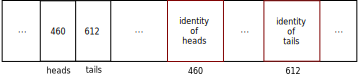
\includegraphics[scale=0.8]{./figures/obj_rep.pdf}
\end{center}

\end{frame}

\begin{frame}[fragile]
\pause

\textbf{Invoking Instance Methods} The purpose of an instance method is to operate on data-type values. We invoke an instance method by writing a variable name that refers to an object, followed by a period, followed by an instance method name, followed by 0 or more arguments, enclosed in parentheses and separated by commas. Eg, 
\begin{lstlisting}[language=Java]
heads.increment();
heads.tally() - tails.tally();

// The following statement implicitly invokes heads.toString() and 
// prints the returned string.
System.out.println(heads); 
\end{lstlisting}

\pause
\smallskip

Eg: Simulating \lstinline$T$ coin flips

\begin{lstlisting}[language=Java]
public class Flips {
    public static void main(String[] args) {
        int T = Integer.parseInt(args[0]);
        Counter heads = new Counter("heads");
        Counter tails = new Counter("tails");
        for (int t = 0; t < T; t++) {
            if (StdRandom.bernoulli(0.5)) {
                heads.increment();
            }
            else {
                tails.increment();
            }
        }
        StdOut.println(heads);
        StdOut.println(tails);
        int delta = heads.tally() - tails.tally();
        StdOut.println("delta: " + Math.abs(delta));
    }
}
\end{lstlisting}
\end{frame}

\begin{frame}[fragile]
\pause

\begin{lstlisting}[language=bash]
$ java Flips 1000000
499422 heads
500578 tails
delta: 1156
\end{lstlisting}

\pause
\smallskip

\textbf{Assignment Statements} An assignment statement with a reference type creates a copy (an alias) of the reference, not a new object. 

\pause
\smallskip

\textbf{Objects as Arguments and Return Values} You can pass objects as arguments to methods and you can also use an object as a return value from a method.

\pause
\smallskip

Eg: Simulating \lstinline$T$ coin flips and finding out who (heads or tails) is the winner

\begin{lstlisting}[language=Java]
public class FlipsMax {
    public static Counter max(Counter x, Counter y) {
        return x.tally() > y.tally() ? x : y;
    }

    public static void main(String[] args) {
        int T = Integer.parseInt(args[0]);
        Counter heads = new Counter("heads");
        Counter tails = new Counter("tails");
        for (int t = 0; t < T; t++) {
            if (StdRandom.bernoulli(0.5)) { heads.increment(); }
            else { tails.increment(); }
        }
        if (heads.tally() == tails.tally()) {
            StdOut.println("Tie");
        }
        else {
            StdOut.println(max(heads, tails) + " wins");
        }
    }
}
\end{lstlisting}

\end{frame}

\begin{frame}[fragile]
\pause

\begin{lstlisting}[language=bash]
$ java FlipsMax 1000000
501181 heads wins
\end{lstlisting}

\pause
\smallskip

\textbf{Arrays and Objects} In Java, every value of any nonprimitive type is an object. In particular, arrays are objects. Array entries can be of any type, including reference types, ie, they can be objects.

\pause
\smallskip

Eg: Simulating \lstinline$T$ rolls of a die

\begin{lstlisting}[language=Java]
public class Rolls {
    public static void main(String[] args) {
        int T = Integer.parseInt(args[0]);
        int SIDES = 6;
        Counter[] rolls = new Counter[SIDES + 1];
        for (int i = 1; i <= SIDES; i++) {
            rolls[i] = new Counter(i + "'s");
        }
        for (int t = 0; t < T; t++) {
            int result = StdRandom.uniform(1, SIDES + 1);
            rolls[result].increment();
        }
        for (int i = 1; i <= SIDES; i++) {
            StdOut.println(rolls[i]);
        }
    }
}
\end{lstlisting}

\pause

\begin{lstlisting}[language=bash]
$ java Rolls 1000000
166674 1's
166337 2's
166566 3's
166926 4's
166822 5's
166675 6's
\end{lstlisting}

\end{frame}

\section{Examples of Abstract Data Types}
\begin{frame}[fragile]
\pause

\textbf{Standard Java System Types in \lstinline$java.lang$}
\begin{lstlisting}[language=Java]
    Integer       // int wrapper
    Double        // double wrapper
    String        // indexed chars
    StringBuilder // builder for strings
\end{lstlisting}

\pause
\smallskip

\textbf{Other Java Types}
\begin{lstlisting}[language=Java]
    java.awt.Color // colors
    java.awt.Font  // fonts
    java.net.URL   // URLs
    java.io.File   // files
\end{lstlisting}

\pause
\smallskip

\textbf{Standard I/O Types from the Text}
\begin{lstlisting}[language=Java]
    In   // input stream
    Out  // output stream
    Draw // drawing
\end{lstlisting}

\pause
\smallskip

\textbf{Data-oriented Types for Client Examples}
\begin{lstlisting}[language=Java]
    Point2D     // point in the plane
    Interval1D  // 1D interval
    Interval2D  // 2D interval
    Date        // date
    Transaction // transaction
\end{lstlisting}

\pause
\smallskip

\textbf{Types for Analysis of Algorithms}
\begin{lstlisting}[language=Java]
    Counter           // counter
    Accumulator       // accumulator
    VisualAccumulator // visual version
    Stopwatch         // stopwatch
\end{lstlisting}
\end{frame}

\begin{frame}[fragile]
\pause

\textbf{Collection Types}
\begin{lstlisting}[language=Java]
    Stack                  // pushdown stack
    Queue                  // FIFO queue
    Bag                    // bag
    MinPQ, MaxPQ           // priority queue
    IndexMinPQ, IndexMaxPQ // priority queue (indexed)
    ST                     // symbol table
    SET                    // set
    StringST               // symbol table (string keys)
\end{lstlisting}

\pause
\smallskip

\textbf{Data-oriented Graph Types}
\begin{lstlisting}[language=Java]
    Graph               // graph
    Digraph             // directed graph
    Edge                // edge (weighted)
    EdgeWeightedGraph   // graph (weighted)
    DirectedEdge        // edge (directed, weighted)
    EdgeWeightedDigraph // graph (directed, weighted)
\end{lstlisting}

\pause
\smallskip

\textbf{Operations-oriented Graph Types}
\begin{lstlisting}[language=Java]
    UF                // dynamic connectivity
    DepthFirstPaths   // DFS path searcher
    CC                // connected components
    BreadhFirstPaths  // BFS path searcher
    DirectedDFS       // DFS digraph path search
    DirectedBFS       // BFS digraph path search
    TransitiveClosure // all paths
    Topological       // topological order
    DepthFirstOrder   // DFS order
    DirectedCycle     // cycle search
    SCC               // strong components
    MST               // minimum spanning tree
    SP                // shortest paths
\end{lstlisting}
\end{frame}

\begin{frame}[fragile]
\pause

\textbf{Geometric Objects} 
\begin{itemize}
\pause

\item An API for points in the plane
\begin{lstlisting}[language=Java]
public class Point2D

    Point2D(double x, double y) // create a point
    double x()                  // x coordinate
    double y()                  // y coordinate
    double r()                  // radius (polar coordinates)
    double theta()              // angle (polar coordinates)
    double distTo(Point2D that) // distance from the point to that
    void draw()                 // draw the point on StdDraw
\end{lstlisting}

\pause

\item An API for intervals on the line
\begin{lstlisting}[language=Java]
public class Interval1D

    Interval1D(double lo, double hi)    // create an interval
    double length()                     // length of the interval
    boolean contains(double x)          // does the interval contain x?
    boolean intersects(Interval1D that) // does the interval intersect that?
    void draw()                         // draw the interval on StdDraw          
\end{lstlisting}

\pause

\item An API for two-dimensional intervals in the plane
\begin{lstlisting}[language=Java]
public class Interval2D
          
    Interval2D(Interval1D x, Interval1D y) // create a 2D interval
    double area()                          // area of the 2D interval 
    boolean contains(Point p)              // does the interval contain p?
    boolean intersects(Interval2D that) // does the interval intersect that?
    void draw()                         // draw the interval on StdDraw
\end{lstlisting}
\end{itemize}
\end{frame}

\begin{frame}[fragile]
\pause 
\begin{itemize}
\item \lstinline$Interval2D$ test client

\begin{lstlisting}[language=Java]
public static void main(String[] args) {
    double xlo = Double.parseDouble(args[0]);
    double xhi = Double.parseDouble(args[1]);
    double ylo = Double.parseDouble(args[2]);
    double yhi = Double.parseDouble(args[3]);
    int T = Integer.parseInt(args[4]);
    Interval1D xinterval = new Interval1D(xlo, xhi);
    Interval1D yinterval = new Interval1D(ylo, yhi);
    Interval2D box = new Interval2D(xinterval, yinterval);
    box.draw();
    Counter counter = new Counter("hits");
    for (int t = 0; t < T; t++) {
        double x = StdRandom.uniform(0.0, 1.0);
        double y = StdRandom.uniform(0.0, 1.0);
        Point2D p = new Point2D(x, y);
        if (box.contains(p)) { counter.increment(); }
        else { p.draw(); }
    }
    StdOut.println(counter);
    StdOut.printf("box area = %.2f\n", box.area());
}
\end{lstlisting}

\pause

\begin{minipage}{160pt}
\begin{lstlisting}[language=bash]
$ java Interval2D 0.2 0.5 0.5 0.6 100000
3092 hits
box area = 0.03
\end{lstlisting}
\end{minipage}%
\begin{minipage}{120pt}
\hfill \includegraphics[scale=0.15]{./figures/interval2D.pdf}
\end{minipage}
\end{itemize}
\end{frame}

\begin{frame}[fragile]
\pause

\textbf{Information Processing} Sample APIs for commercial applications (dates and transactions)
\begin{itemize}
\pause

\item API for dates
\begin{lstlisting}[language=Java]
public class Date implements Comparable<Date>

    Date(int month, int day, int year) // create a date
    Date(String date)                  // create a date (parse constructor)
    int month()                        // month
    int day()                          // day
    int year()                         // year
    String toString()                  // string representation
    boolean equals(Object that)        // is the date same as that?
    int compareTo(Date that)           // compare the date to that
    int hashCode()                     // hash code
\end{lstlisting}

\pause

\item API for transactions
\begin{lstlisting}[language=Java]
public class Transaction implements Comparable<Transaction>

    Transaction(String who, Date when, double amount) // create a 
                                                      // transaction
    Transaction(String transaction) // create a transaction 
                                    // (parse constructor)
    String who()                    // customer name
    Date when()                     // date
    double amount()                 // amount
    String toString()               // string representation
    boolean equals(Object that)     // is the transaction same as that?
    int compareTo(Transaction that) // compare the transaction to that
    int hashCode()                  // hash code
\end{lstlisting}
\end{itemize}

\end{frame}

\begin{frame}[fragile]
\pause

\textbf{Strings} Java \lstinline$String$ API (partial list of methods)

\begin{lstlisting}[language=Java]
public class String implements Comparable<String>

    String()                     // create an empty string
    int length()                 // length of the string
    int charAt(int i)            // ith character
    int indexOf(String p)        // first occurrence of p (-1 if none)
    int indexOf(String p, int i) // first occurrence of p after i (-1 if none)
    String concat(String t)        // the string with t appended
    String substring(int i, int j) // substring of the string (i to j - 1)
    String[] split(String delim)   // strings between occurrences of delim
    int compareTo(String t)        // string comparison
    boolean equals(String t)       // is the string's value the same as t's?
    int hashCode()                 // hash code
\end{lstlisting}

\pause
\smallskip

\textbf{Input and Output Revisited} A disadvantage of the \lstinline$StdIn$, \lstinline$StdOut$, and \lstinline$StdDraw$ is that they restrict us to working with just one input file, one output file, and one drawing for any given program. With object-oriented programming, we can define similar mechanisms that allow us to work with multiple input streams, output streams, and drawings within one program.

\begin{itemize}
\pause

\item API for a data type for input streams

\begin{lstlisting}[language=Java]
public class In

    In()                // create an input stream from standard input
    In(String name)     // create an input stream from a file or website
    ...
    void close()        // close the input stream
\end{lstlisting}

\end{itemize}
\end{frame}

\begin{frame}[fragile]
\pause

\begin{itemize}
\item API for a data type for output streams
\begin{lstlisting}[language=Java]
public class Out

    Out()                   // create an output stream to standard output
    Out(String name)        // create an output stream to a file
    ...
    void close()            // close the output stream
\end{lstlisting}

\pause

\item A sample \lstinline$In$ and \lstinline$Out$ client
\begin{lstlisting}[language=Java]
public class Cat { 
   public static void main(String[] args) { 
        Out out = new Out(args[args.length - 1]);
        for (int i = 0; i < args.length - 1; i++) {
            In in = new In(args[i]);
            String s = in.readAll();
            out.println(s);
            in.close();
        }
        out.close();
    }
}
\end{lstlisting}

\pause

\begin{lstlisting}[language=bash]
$ more A.txt
To be, or not to be, that is the question
$ java Cat A.txt B.txt
$ more B.txt
To be, or not to be, that is the question.
\end{lstlisting}

\pause

\item API for a data type for drawing
\begin{lstlisting}[language=Java]
public class Draw

    Draw()
    void line(double x0, double y0, double x1, double y1)
    ...
\end{lstlisting}
\end{itemize}
\end{frame}

\section{Implementing an Abstract Data Type}
\begin{frame}[fragile]
\pause

We implement ADTs with a Java class, putting the code (instance variable declarations, constructors, and instance methods) in a file with the same name as the class, followed by the \lstinline$.java$ extension. 

\pause
\smallskip

\textbf{Instance Variables} Define the state of each object. Unlike local variables, each instance variable can have numerous values (one per object).

\pause
\smallskip

\textbf{Constructors} Are like static methods, but they can refer directly to instance variables and have no return value. Generally, their purpose is initialize the instance variables. Every constructor creates an object and provides to the client a reference to that object.

\pause
\smallskip

\textbf{Instance Methods} They define the behavior of each object. Each instance method has a return type, a signature, and a body. When a client invokes an instance method (eg, \lstinline$heads.increment()$), the action is the same as for
static methods, with one critical distinction: they can access
and perform operations on instance variables. Within an instance method or a constructor, \lstinline$this$ is a reference to the current object --- the object whose method or constructor is being called. The most common reason for using the \lstinline$this$ keyword is because a field (instance variable) is shadowed by a method or constructor parameter.
\end{frame}

\begin{frame}[fragile]
\pause

\textbf{Counter}
\begin{itemize}
\item API
\begin{lstlisting}[language=Java]
public class Counter

    Counter(String id) // create a counter named id
    void increment()   // increment the counter by one
    int tally()        // number of increments since creation
    String toString()  // string representation
\end{lstlisting}

\pause
\item Typical client
\begin{lstlisting}[language=Java]
public class Flips {
    public static void main(String[] args) {
        int T = Integer.parseInt(args[0]);
        Counter heads = new Counter("heads");
        Counter tails = new Counter("tails");
        for (int t = 0; t < T; t++) {
            if (StdRandom.bernoulli(0.5)) {
                heads.increment();
            }
            else {
                tails.increment();
            }
        }
        StdOut.println(heads);
        StdOut.println(tails);
        int delta = heads.tally() - tails.tally();
        StdOut.println("delta: " + Math.abs(delta));
    }
}
\end{lstlisting}

\begin{lstlisting}[language=bash]
$ java Flips 1000000
499422 heads
500578 tails
delta: 1156
\end{lstlisting}
\end{itemize}
\end{frame}

\begin{frame}[fragile]
\pause

\begin{itemize}
\item Implementation
\begin{lstlisting}[language=Java]
public class Counter {
    private final String name;
    private int count;

    public Counter(String id) { 
        name = id; 
    }

    public void increment() { 
        count++; 
    }

    public int tally() { 
        return count; 
    }

    public String toString() { 
        return count + " " + name; 
    }
}
\end{lstlisting}
\end{itemize}
\end{frame}

\begin{frame}[fragile]
\pause

\textbf{Date}
\begin{itemize}
\item API
\begin{lstlisting}[language=Java]
public class Date implements Comparable<Date>

    Date(int month, int day, int year) // create a date
    int month()                        // month
    int day()                          // day
    int year()                         // year
    String toString()                  // string representation
\end{lstlisting}

\pause
\item Typical client
\begin{lstlisting}[language=Java]
public class Date {
    ...
    
    public static void main(String[] args) {
        int m = Integer.parseInt(args[0]);
        int d = Integer.parseInt(args[1]);
        int y = Integer.parseInt(args[2]);
        Date date = new Date(m, d, y);
        StdOut.println(date);
    }
}
\end{lstlisting}

\begin{lstlisting}[language=bash]
$ java Date 12 31 1999
12/31/1999
\end{lstlisting}
\end{itemize}
\end{frame}

\begin{frame}[fragile]
\pause

\begin{itemize}
\item Implementation
\begin{lstlisting}[language=Java]
public class Date {
    private final int month;
    private final int day;
    private final int year;
    
    public Date(int m, int d, int y) { 
        month = m; 
        day = d; 
        year = y; 
    }
    
    public int month() { 
        return month; 
    }

    public int day() { 
        return day; 
    }

    public int year() { 
        return year; 
    }
    
    public String toString() { 
        return month() + "/" + day() + "/" + year();
    }
}
\end{lstlisting}
\end{itemize}
\end{frame}

\begin{frame}[fragile]
\pause

\textbf{Accumulator} An abstract data type that provides clients the ability to maintain a running average of data values.
\begin{itemize}
\item API
\begin{lstlisting}[language=Java]
public class Accumulator

    Accumulator()                 // create an accumulator
    void addDateValue(double val) // add a new data value
    double mean()                 // mean of all data values
    String toString()             // string representation
\end{lstlisting}

\pause
\item Typical client
\begin{lstlisting}[language=Java]
public class TestAccumulator {
    public static void main(String[] args) {
        int T = Integer.parseInt(args[0]);
        Accumulator a = new Accumulator();
        for (int t = 0; t < T; t++) {
            a.addDataValue(StdRandom.random());
        }
        StdOut.println(a);
    }
}
\end{lstlisting}

\begin{lstlisting}[language=bash]
$ java TestAccumulator 1000
Mean (1000 values): 0.50832
$ java TestAccumulator 1000000
Mean (1000000 values): 0.49970
$ java TestAccumulator 1000000
Mean (1000000 values): 0.49976
\end{lstlisting}
\end{itemize}
\end{frame}

\begin{frame}[fragile]
\pause

\begin{itemize}
\item Implementation
\begin{lstlisting}[language=Java]
public class Accumulator {
    private double total;
    private int N;

    public void addDataValue(double val) {
        N++;
        total += val;
    }

    public double mean() {
        return total / N;
    }

    public String toString() {
        return "Mean (" + N + " values): " + String.format("%7.5f", mean());
    }
}
\end{lstlisting}
\end{itemize}
\end{frame}

\begin{frame}[fragile]
\pause

\textbf{Visual Accumulator} The visual accumulator implementation extends accumulator to present a useful side effect: it draws on \lstinline$StdDraw$ all the data (in gray) and the running average (in red).
\begin{itemize}
\item API
\begin{lstlisting}[language=Java]
public class VisualAccumulator

    VisualAccumulator(int trials, double max) // create a visual accumulator
    void addDateValue(double val)             // add a new data value
    double mean()                             // mean of all data values
    String toString()                         // string representation
\end{lstlisting}

\pause
\item Typical client
\begin{lstlisting}[language=Java]
public class TestVisualAccumulator {
    public static void main(String[] args) {
        int T = Integer.parseInt(args[0]);
        VisualAccumulator a = new VisualAccumulator(T, 1.0);
        for (int t = 0; t < T; t++) {
            a.addDataValue(StdRandom.random());
        }
        StdOut.println(a);
    }
}
\end{lstlisting}

\begin{minipage}{160pt}
\begin{lstlisting}[language=bash]
$ java TestVisualAccumulator 10000
Mean (10000 values):  0.49558
\end{lstlisting}
\end{minipage}%
\begin{minipage}{120pt}
\hfill \includegraphics[scale=0.13]{./figures/visual_acc.pdf}
\end{minipage}
\end{itemize}
\end{frame}

\begin{frame}[fragile]
\pause

\begin{itemize}
\item Implementation
\begin{lstlisting}[language=Java]
public class VisualAccumulator {
    private double total;
    private int N;

    public VisualAccumulator(int trials, double max) {
        StdDraw.setXscale(0, trials);
        StdDraw.setYscale(0, max);
        StdDraw.setPenRadius(.005);
    }

    public void addDataValue(double val) {
        N++;
        total += val;
        StdDraw.setPenColor(StdDraw.DARK_GRAY);
        StdDraw.point(N, val);
        StdDraw.setPenColor(StdDraw.RED);
        StdDraw.point(N, mean());
    }

    public double mean() {
        return total / N;
    }

    public String toString() {
        return "Mean (" + N + " values): " + String.format("%7.5f", mean());
    }
}
\end{lstlisting}
\end{itemize}
\end{frame}

\section{Data-type Design}
\begin{frame}[fragile]
\pause

\textbf{Encapsulation} Enables modular programming, allowing us to
\begin{itemize}
\item Independently develop client and implementation code; 
\item Substitute improved implementations without affecting clients; and
\item Support programs not yet written (the API is a guide for any future client).
\end{itemize}

\pause
\smallskip

\textbf{Designing APIs} Consider writing every program as though you
will need to reuse the code someday. Articulate an API for your program, providing to clients only the methods they need and no others. 

\pause
\smallskip

\textbf{Algorithms and ADTs} Data abstraction provides a natural framework for precisely specifying both what an algorithm needs to accomplish and how a client can make use of the algorithm. 

\pause
\smallskip

Eg: Binary search as an ADT (\lstinline$StaticSETofInts$) for searching a set of integers

\pause
\smallskip

\begin{itemize}
\item API for \lstinline$StaticSETofInts$
\begin{lstlisting}[language=Java]
public class StaticSETofInts

    StaticSETofInts(int[] a)  // create a set from the values in a
    boolean contains(int key) // is key in the set? 
\end{lstlisting}
\end{itemize}
\end{frame}

\begin{frame}[fragile]
\pause

\begin{itemize}
\item Typical client
\begin{lstlisting}[language=Java]
public class Whitelist {
    public static void main(String[] args) {
        In in = new In(args[0]);
        int[] white = in.readAllInts();
        StaticSETofInts set = new StaticSETofInts(white);
        while (!StdIn.isEmpty()) {
            int key = StdIn.readInt();
            if (!set.contains(key)) {
                StdOut.println(key);
            }
        }
    }
}
\end{lstlisting}

\pause

\begin{lstlisting}[language=Java]
$ java Whitelist largeW.txt < largeT.txt
499569
984875
295754
207807
140925
161828
...
\end{lstlisting}

\end{itemize}
\end{frame}

\begin{frame}[fragile]
\pause

\begin{itemize}
\item Implementation
\begin{lstlisting}[language=Java]
import java.util.Arrays;

public class StaticSETofInts {
    private int[] a;
   
    public StaticSETofInts(int[] keys) {
        a = new int[keys.length];
        for (int i = 0; i < keys.length; i++) {
            a[i] = keys[i]; 
        }
        Arrays.sort(a);
    }
    
    public boolean contains(int key) { 
        return rank(key) != -1; 
    }

    private int rank(int key) { 
        int lo = 0;
        int hi = a.length - 1;
        while (lo <= hi) { 
            int mid = lo + (hi - lo) / 2;
            if (key < a[mid]) { hi = mid - 1; }
            else if (key > a[mid]) { lo = mid + 1; }
            else { return mid; }
        }
        return -1;
    }
}
\end{lstlisting}
\end{itemize}
\end{frame}

\begin{frame}[fragile]
\pause

\textbf{Interface Inheritance (aka Subtyping)} Allows us to specify a relationship between otherwise unrelated classes by specifying in
an interface a set of common methods that each implementing class must contain. 

\pause
\smallskip

Comparison interfaces (\lstinline$java.lang.Comparable$ and \lstinline$java.util.Comparator$)
\begin{lstlisting}[language=Java]
public interface Comparable<T>

    int compareTo(T o) // compares the object with o for order
\end{lstlisting}

\begin{lstlisting}[language=Java]
public interface Comparator<T>

    int compare(T o1, T o2)  // compares o1 and o2 for order
    boolean equals(Object o) // is the comparator equal to o? 
\end{lstlisting}

\pause

Eg: Data type for a planet

\begin{lstlisting}[language=Java]
public class Planet implements Comparable<Planet> {
    private String name;
    private int moons;

    public Planet(String name, int moons) {
        this.name = name;
        this.moons = moons;
    }
    
    public String name() { return name; }

    public int moons() { return moons; }

    public int compareTo(Planet o) { return name.compareTo(o.name); }
    
    public String toString() { return name + ", " + moons; }
}
\end{lstlisting}
\end{frame}

\begin{frame}[fragile]
\pause

\begin{lstlisting}[language=Java]
import java.util.Comparator;

public class MoonComparator implements Comparator<Planet> {
    public int compare(Planet p1, Planet p2) { return p1.moons() - p2.moons(); }
    
    public boolean equals(Object o){ return o instanceof MoonComparator; }
}
\end{lstlisting}

\begin{lstlisting}[language=Java]
import java.util.Arrays;

public class PlanetTester {
    public static void main(String[] args) {
        Planet[] planets = new Planet[8];
        planets[0] = new Planet("Mercury", 0);
        planets[1] = new Planet("Venus", 0);
        planets[2] = new Planet("Earth", 1);
        planets[3] = new Planet("Mars", 2);
        planets[4] = new Planet("Jupiter", 67);
        planets[5] = new Planet("Saturn", 62);
        planets[6] = new Planet("Uranus", 27);
        planets[7] = new Planet("Neptune", 14);
        System.out.println("Unsorted:");
        for (Planet p : planets) { System.out.println("  " + p); }
        Arrays.sort(planets);
        System.out.println("Sorted by name:");
        for (Planet p : planets) { System.out.println("  " + p); }
        Arrays.sort(planets, new MoonComparator());
        System.out.println("Sorted by # of moons:");
        for (Planet p : planets) { System.out.println("  " + p); }
    }
}
\end{lstlisting}
\end{frame}

\begin{frame}[fragile]
\pause

\begin{lstlisting}[language=Java]
$ java PlanetTester 
Unsorted:
  Mercury, 0
  Venus, 0
  Earth, 1
  Mars, 2
  Jupiter, 67
  Saturn, 62
  Uranus, 27
  Neptune, 14
Sorted by name:
  Earth, 1
  Jupiter, 67
  Mars, 2
  Mercury, 0
  Neptune, 14
  Saturn, 62
  Uranus, 27
  Venus, 0
Sorted by # of moons:
  Mercury, 0
  Venus, 0
  Earth, 1
  Mars, 2
  Neptune, 14
  Uranus, 27
  Saturn, 62
  Jupiter, 67
\end{lstlisting}
\end{frame}

\begin{frame}[fragile]
\pause

Iteration interfaces (\lstinline$java.lang.Iterable$ and \lstinline$java.util.Iterator$)
\begin{lstlisting}[language=Java]
public interface Iterable<T>

    Iterator<T> iterator() // an iterator over a set of elements of type T
\end{lstlisting}

\begin{lstlisting}[language=Java]
public interface Iterator<E>

    boolean hasNext() // does the iteration have more elements?
    E next()          // next element in the iteration
    void remove()     // remove the last element returned
\end{lstlisting}

An iterable type (arrays included) can be enumerated using the enhanced \lstinline$for$ statement. Eg, the following code 

\begin{lstlisting}[language=Java]
String[] dow = {"Sun", "Mon", "Tue", "Wed", "Thu", "Fri", "Sat"};
for (String s : dow) {
    StdOut.println(s);
}
\end{lstlisting}

would output

\begin{lstlisting}[language=Java]
Sun
Mon
Tue
Wed
Thu
Fri
Sat
\end{lstlisting}
\end{frame}

\begin{frame}[fragile]
\pause

Eg: An iterator for the Fibonacci sequence

\begin{lstlisting}[language=Java]
import java.util.Iterator;

public class Fibonacci implements Iterable<Long> {
    private int n;

    public Fibonacci(int n) { this.n = n; }

    public Iterator<Long> iterator() { return new FibonacciIterator(); }

    private class FibonacciIterator implements Iterator<Long> {
        private int count = 0;
        private long a = 1, b = 1;

        public boolean hasNext() { return count <= n; }

        public Long next() {
            count++;
            if (count <= 2) { return (long) 1; }
            else { 
                long t = b; b = a + b; a = t;
                return b;
            }
        }
        
        public void remove() {}
    }

    public static void main(String[] args) {
        int n = Integer.parseInt(args[0]);
        for (long i : new Fibonacci(n)) {
            StdOut.println(i);
        }
    }
}
\end{lstlisting}
\end{frame}

\begin{frame}[fragile]
\pause

\begin{lstlisting}[language=bash]
$ java Fibonacci 10
1
1
2
3
5
8
13
21
34
55
89
\end{lstlisting}

\pause
\smallskip

\textbf{Implementation Inheritance (aka Subclassing)} Enables a programmer to change behavior and add functionality without rewriting an entire class from scratch, by defining a new class (subclass or derived class) that inherits instance methods and instance variables from another class (superclass or base class). 

\pause
\smallskip

Every class in Java is a subclass of the \lstinline$java.lang.Object$ class and therefore inherits its methods, some which are:

\begin{lstlisting}[language=Java]
public class Object
    
    Class getClass()            // what class is the object?
    String toString()           // string representation of the object
    boolean equals(Object that) // is the object equal to that?
    int hashCode()              // hash code for the object
\end{lstlisting}

\end{frame}

\begin{frame}[fragile]
\pause

\textbf{String Conversion} Since every Java type inherits \lstinline$toString()$ from \lstinline$Object$, any client can invoke \lstinline$toString()$ for any object. If an object's data type does not include an implementation of \lstinline$toString()$, then the default implementation in \lstinline$Object$ is invoked,
which returns the memory address of the object. We generally include implementations of \lstinline$toString()$ that override the default in every class that we develop.

\pause
\smallskip

\textbf{Wrapper Types} Reference types provided by Java for each of the primitive types (eg, \lstinline$Boolean$ for \lstinline$boolean$, \lstinline$Integer$ for \lstinline$int$, etc). Java automatically converts primitive types to wrapper types (auto boxing) and wrapper types to primitive types (auto unboxing).

\pause
\smallskip

\textbf{Equality} If we test equality with \lstinline$a == b$ where \lstinline$a$ and \lstinline$b$ are reference variables of the same type, we are testing whether they have the same identity, ie, the same address. We must instead use \lstinline$a.equals(b)$. When we define our own data type, we must override the \lstinline$equals()$ method inherited from \lstinline$Object$.

\pause
\smallskip

\textbf{Memory Management} The ability to assign a new value to a reference variable can lead to orphaned objects. Eg, the object representing the date Jan 1, 2015 is orphaned in the following example

\begin{lstlisting}[language=Java]
Date a = new Date(12, 31, 2014);
Date b = new Date(1, 1, 2015);
b = a;
\end{lstlisting}

One of Java's most significant features is its ability to automatically manage memory (known as \emph{garbage collection}) by keeping track of orphaned objects and returning the memory they use to a pool of free memory. 

\end{frame}

\begin{frame}[fragile]
\pause

\textbf{Immutability} An immutable data type (eg, \lstinline$Date$) has the property that the value of an object never changes once constructed. Java enforces immutability via the \lstinline$final$ modifier; a variable declared to be \lstinline$final$ can be assigned a value only once, either in an initializer or in the constructor.

\pause
\smallskip

\textbf{Exceptions and Errors} Exceptions and errors are disruptive events that occur while a program is running. We have encountered exceptions thrown by Java system methods, such as   \lstinline$StackOverflowError$, \lstinline$ArithmeticException$, \lstinline$ArrayIndexOutOfBoundsException$, \lstinline$OutOfMemoryError$, and \lstinline$NullPointerException$. We can also raise exceptions within a program, the simplest being a \lstinline$RuntimeException$ that terminates execution of the program and prints an error message.

\begin{lstlisting}[language=Java]
throw new RuntimeException("Error message here.");
\end{lstlisting}

\pause
\smallskip

\textbf{Assertions} A Boolean expression that we are affirming is true at that point in the program. If the expression is \lstinline$false$, the program will terminate and report an error message. Eg,

\begin{lstlisting}[language=Java]
assert index >= 0;
\end{lstlisting}

or the following with a custom message

\begin{lstlisting}[language=Java]
assert index >= 0 : "Negative index in method X";
\end{lstlisting}
\end{frame}

\end{document}
